\section{类和对象}
\hfill\ctli{实验时间}{~2014~年~11~月~29~日}
\subsection*{【实验目的】}
\begin{enumerate}[topsep=0pt,partopsep=0pt,itemsep=0pt,parsep=0pt,label={\arabic*、}]
\item 掌握类、对象、数据成员、成员函数的基本概念。
\item 能够进行类的定义。
\item 能够使用成员函数进行相关调用。
\end{enumerate}
\subsection*{【实验环境】}
\MyEnvironment
\subsection*{【实验内容】}
\begin{enumerate}[topsep=0pt,partopsep=0pt,itemsep=0pt,parsep=0pt,label={\arabic*、}]
\item 编写NumberA类,实现两个整数的加减乘除运算。构造函数实现两整数a,b赋值。
\item 编写OperaN类,实现输入1.2.3.4解析成加减乘除符号。
\item P89:3.11
\end{enumerate}

\subsection{NumberA 类}
\subsubsection*{【详细分析】}
NumberA 类设有两个成员变量存放两个操作数,提供对这两个操作数进行四则运算的方法。
\subsubsection*{【实验源码】}
{\linespread{1}\lstinputlisting[caption={\tt exp01.cpp}]{exp02/exp01.cpp}}
\subsubsection*{【实验结果】}
\begin{figure}[htp]
\centering
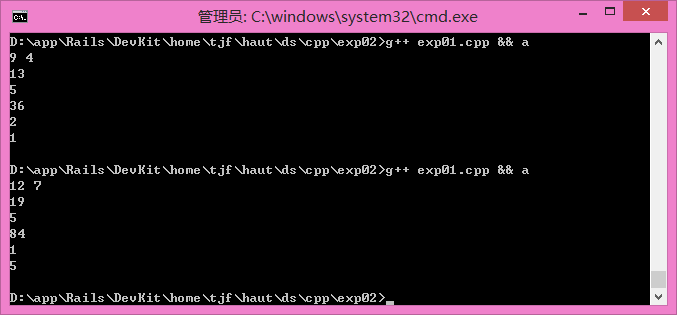
\includegraphics[width=\textwidth]{exp02/exp01.png}
\caption{\label{out02_01}NumberA 类}
\end{figure}

\subsection{OperaN 类}
\subsubsection*{【详细分析】}
用一个整数初始化类,置符号。
\subsubsection*{【实验源码】}
{\linespread{1}\lstinputlisting[caption={\tt exp02.cpp}]{exp02/exp02.cpp}}
\subsubsection*{【实验结果】}
\begin{figure}[htp]
\centering
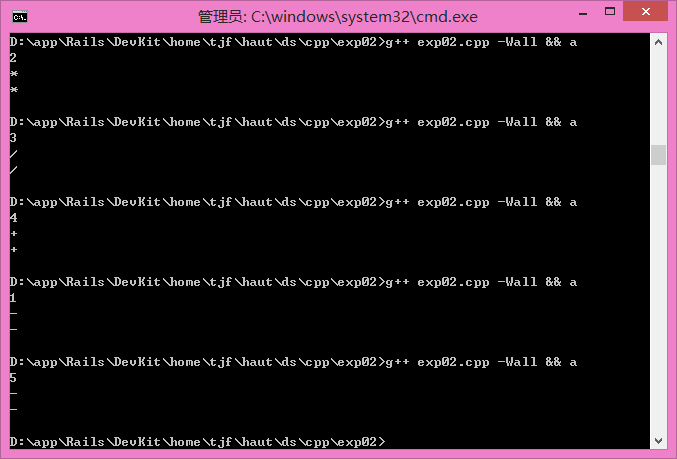
\includegraphics[width=\textwidth]{exp02/exp02.png}
\caption{\label{out02_02}OperaN 类}
\end{figure}

\subsection{P89:3.11}
\subsubsection*{【详细分析】}
对 Account 类的修改。
\subsubsection*{【实验源码】}
{\linespread{1}\lstinputlisting[caption={\tt GradeBook.h}]{exp02/GradeBook.h}}
{\linespread{1}\lstinputlisting[caption={\tt GradeBook.cpp}]{exp02/GradeBook.cpp}}
{\linespread{1}\lstinputlisting[caption={主程序 \tt exp03.cpp}]{exp02/exp03.cpp}}
\subsubsection*{【实验结果】}
\begin{figure}[htp]
\centering
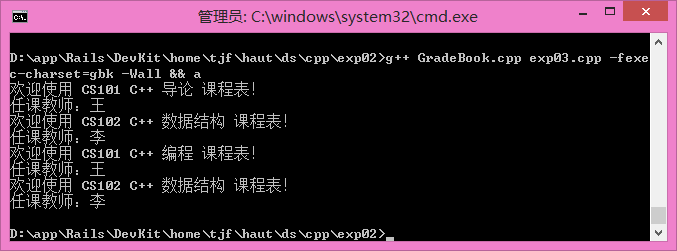
\includegraphics[width=\textwidth]{exp02/exp03.png}
\caption{\label{out02_03}P89:3.11}
\end{figure}

\subsection*{【实验体会】}
(至少150字)